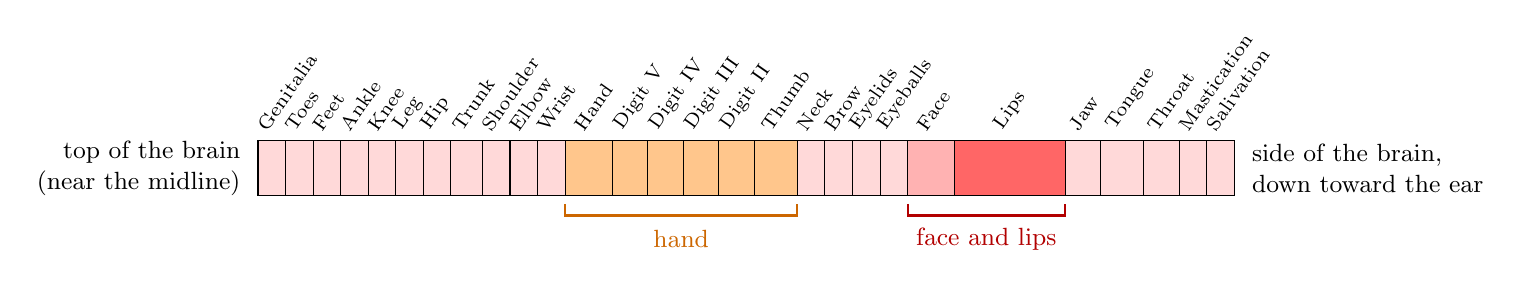
\begin{tikzpicture}[font=\scriptsize]
  % body map along the cortical strip, unrolled: from the top of the brain (left) down the side (right)
  % entries: label / width / color
  \def\pos{0}
  \foreach \lab/\w/\c in {
      Genitalia/0.35/red!15, Toes/0.35/red!15, Feet/0.35/red!15, Ankle/0.35/red!15,
      Knee/0.35/red!15, Leg/0.35/red!15, Hip/0.35/red!15, Trunk/0.4/red!15,
      Shoulder/0.35/red!15, Elbow/0.35/red!15, Wrist/0.35/red!15,
      Hand/0.6/orange!45, Digit V/0.45/orange!45, Digit IV/0.45/orange!45,
      Digit III/0.45/orange!45, Digit II/0.45/orange!45, Thumb/0.55/orange!45,
      Neck/0.35/red!15, Brow/0.35/red!15, Eyelids/0.35/red!15, Eyeballs/0.35/red!15,
      Face/0.6/red!30, Lips/1.4/red!60, Jaw/0.45/red!15, Tongue/0.55/red!15,
      Throat/0.45/red!15, Mastication/0.35/red!15, Salivation/0.35/red!15} {
    \filldraw[fill=\c, draw=black] (\pos,0) rectangle ++(\w,0.7);
    \node[anchor=south west, rotate=55, inner sep=1pt] at ({\pos+\w/2-0.05},0.75) {\lab};
    \pgfmathparse{\pos+\w}\xdef\pos{\pgfmathresult}
  }
  % ends of the strip
  \node[anchor=east, align=right, font=\small] at (-0.1,0.35) {top of the brain\\(near the midline)};
  \node[anchor=west, align=left, font=\small] at ({\pos+0.1},0.35) {side of the brain,\\down toward the ear};
  % neighbors
  \draw[thick, orange!80!black] (3.9,-0.1) -- (3.9,-0.25) -- (6.85,-0.25) -- (6.85,-0.1);
  \node[orange!80!black, font=\small] at (5.375,-0.55) {hand};
  \draw[thick, red!70!black] (8.25,-0.1) -- (8.25,-0.25) -- (10.25,-0.25) -- (10.25,-0.1);
  \node[red!70!black, font=\small] at (9.25,-0.55) {face and lips};
\end{tikzpicture}
